\documentclass[12pt,a4paper]{article}

\usepackage[utf8]{inputenc}
\usepackage[T1]{fontenc}
\usepackage[brazil]{babel}
\usepackage{graphicx}
\usepackage{amsmath}
\usepackage{geometry}
\usepackage{setspace}
\usepackage{float}
\usepackage{listings}
\usepackage{algorithm}
\usepackage{algorithmic}
\usepackage{subcaption}
\usepackage[style=numeric,backend=biber]{biblatex}
\usepackage{kpfonts}
\usepackage{wrapfig}
\usepackage{enumerate}
\usepackage{caption}
\usepackage{lipsum}
\usepackage{amsthm}
\usepackage{amssymb}
\usepackage{bm}
\usepackage{color}
\usepackage{afterpage}
\usepackage[inline]{enumitem}
\usepackage{pdflscape}
\usepackage{listingsutf8}
\usepackage{siunitx}
\usepackage{bashful}
\usepackage[hidelinks]{hyperref}

% Definindo estilo para os códigos
\definecolor{mGreen}{rgb}{0,0.6,0}
\definecolor{mGray}{rgb}{0.5,0.5,0.5}
\definecolor{mPurple}{rgb}{0.58,0,0.82}
\definecolor{dkgreen}{rgb}{0,0.6,0}
\definecolor{backgroundColour}{rgb}{0.97,0.97,0.97}

\lstset{basicstyle=\ttfamily,
    backgroundcolor=\color{backgroundColour},   
    commentstyle=\color{mGreen},
    keywordstyle=\color{magenta},
    numberstyle=\tiny\color{mGray},
    commentstyle=\color{dkgreen},
    stringstyle=\color{mPurple},
    basicstyle=\footnotesize,
    breakatwhitespace=false\textbf{,}         
    breaklines=true,                 
    captionpos=b,                    
    keepspaces=true,                 
    numbers=left,                    
    numbersep=5pt,                  
    showspaces=false,                
    showstringspaces=false,
    showtabs=false,                  
    tabsize=2,
    language=bash
}

\lstdefinestyle{BStyle}{
    backgroundcolor=\color{backgroundColour},  
    showstringspaces=false,
    numbers=none,
    language=bash
}

\geometry{left=2.5cm, right=2.5cm, top=2.5cm, bottom=2.5cm}
\onehalfspacing

\begin{document}

\begin{center}
    \Large \textbf{Universidade Estadual de Campinas} \\
    \large Instituto de Computação \\
    \vspace{0.5cm}
    \large Introdução ao Processamento Digital de Imagens (MC920 / MO443) \\
    \large Professor: Hélio Pedrini
\end{center}

\vspace{2cm}

\begin{center}
    \LARGE \textbf{Trabalho 2} \\
    \vspace{0.5cm}
    \Large Julio Vinicius Amaral Oliveira – 230537
\end{center}

\vspace{2cm}

\begin{flushright}
    \large \textbf{Data de Entrega:} 28 de Abril de 2025
\end{flushright}

\newpage

\section*{Introdução}
O seguinte trabalho visa demonstrar o uso das técnicas de meios-tons e filtragem no domínio da frequência. Para o exercício 1, vamos usar um algoritmo de difusão de erro para quantizar os níveis de cinza de uma imagem, nosso intuito é preservar a percepção visual da imagem mesmo reduzindo a quantidade de tons de cinza dela. No segundo exercício, vamos utilizar a Transformada Rápida de Fourier para realizar operações como suavização, realce de bordas e compressão de dados. 

\section{Materiais e métodos}
Para a resolução dos exercícios propostos, utilizamos as bibliotecas:
\begin{itemize}
    \item \texttt{OpenCV}: Utilizada para ler, processar e exibir imagens.
    \item \texttt{Numpy}: Responsável pelo tratamento dos dados das imagens como arrays. É usada para realizar operações matemáticas, tanto as elementares como multiplicação e potenciação, quanto as mais complexas como a transformada de Fourier. Além de manipulação dos pixels de forma vetorizada, que é fundamental para o processamento de imagens de forma performática.
    \item \texttt{matplotlib}: Utilizado para a visualização das imagens no ambiente do Jupyter Notebook.
\end{itemize}

As atividades desenvolvidas foram organizadas em dois notebooks distintos, denominados \texttt{Parte1.ipynb} e \texttt{Parte2.ipynb}. No primeiro, abordamos as técnicas de meios-tons com difusão de erro. No segundo, aplicamos filtragem no domínio da frequência através da Transformada Rápida de Fourier, implementando filtros passa-baixa, passa-alta, passa-faixa e rejeita-faixa, bem como procedimentos de compressão por limiarização de coeficientes.

\section{Códigos auxiliares}
Para a resolução dos desafios propostos, utilizamos um código auxiliar que serviu para encapsular a lógica de uma sequência de comandos. O código auxiliar criado foi:

\begin{lstlisting}[language=Python, caption={Funções auxiliares para visualização de imagens}]
def print_mono_image(image, title):
    plt.imshow(image, cmap='gray')
    if (title is not None):
        plt.title(title)
    plt.axis('off')
    plt.show()
\end{lstlisting}

\section{Exercícios e Discussão}

\subsection{Exercício 1 – Técnicas de Meios-Tons com Difusão de Erro}

Neste exercício, vamos aplicar técnicas de meios-tons com difusão de erro em imagens digitais carregadas do diretório exttt{../imagens/}. Implementamos os métodos de Floyd-Steinberg, Burkes, Jarvis-Judice-Ninke, Sierra, Stevenson-Arce e Stucki. Cada algoritmo distribui o erro de quantização a pixels vizinhos segundo matrizes de pesos distintas.

\subsubsection*{Estruturas de Dados}
As imagens foram representadas como \texttt{numpy.ndarray} bidimensionais. De modo a garantir precisão na propagação do erro, convertemos os valores de pixel para \texttt{float64}. Após aplicar a difusão, reconvertemos para \texttt{uint8} para gerar as imagens finais.

Adicionalmente, as máscaras de difusão de erro foram armazenadas em um dicionário Python (\texttt{error\_diffusion\_masks}), em que cada chave é o nome do método e cada valor é uma lista de tuplas \texttt{(i\_rel, j\_rel, peso)}, por exemplo:

\begin{lstlisting}[language=Python, caption={Exemplo de definição das máscaras}]
error_diffusion_masks = {
    "Floyd Steinberg": [
        (0,  1, 7/16),
        (1, -1, 3/16),
        (1,  0, 5/16),
        (1,  1, 1/16),
    ]
}
\end{lstlisting}

Esse formato facilitou a criação de uma função genérica, usada tanto na varredura unidirecional quanto na serpentina, tornando o código muito mais elegante, pois para obter o resultado de todos os filtros, nós precisamos apenas iterar através de todas as máscaras.


\subsubsection*{Metodologia}
Para implementar as técnicas de difusão de erro, desenvolvemos duas funções genéricas em Python, sendo que ambas recebem como parâmetros o caminho da imagem e a máscara de difusão (tuplas \texttt{(i\_rel, j\_rel, peso)}) extraída de \texttt{error\_diffusion\_masks}:
\begin{itemize}
  \item \textbf{Leitura e preparo da imagem:}
    \begin{enumerate}
      \item Carregamos a imagem em escala de cinza 
    \end{enumerate}
  \item \textbf{Varredura unidirecional (\texttt{apply\_dithering\_unidirectional}):}
    \begin{enumerate}
      \item Percorremos cada pixel $(i,j)$ em ordem crescente de linhas e colunas.
      \item Binarizamos: \texttt{out\_image[i,j] = 0} se \texttt{image[i,j] < 128} senão \texttt{255}.
      \item Calculamos o erro: \texttt{error = image[i,j] - out\_image[i,j]}.
      \item Para cada tupla da máscara, distribuímos \texttt{error * peso} a \texttt{image[i+i\_rel, j+j\_rel]}, caso as posições estivessem dentro dos limites da imagem.
    \end{enumerate}
  \item \textbf{Varredura em serpentina (\texttt{apply\_serpentine\_scanning}):}
    \begin{enumerate}
      \item Alternamos a direção de varredura a cada linha: colunas esquerda→direita em linhas pares, direita→esquerda em linhas ímpares.
      \item Ajustamos o deslocamento horizontal do erro (\texttt{j\_rel}) invertendo seu sinal quando a linha é ímpar, para manter a matriz de difusão centrada corretamente.
      \item O restante do fluxo é idêntico ao método unidirecional (binarização, cálculo de erro, distribuição).
    \end{enumerate}
  \item \textbf{Visualização e validação:}
    \begin{enumerate}
      \item Após a execução de cada método, exibimos \texttt{original}, \texttt{unidirectional} e \texttt{serpentine} lado a lado via \texttt{matplotlib.pyplot.subplots}.
      \item Os resultados foram salvos em \texttt{../resultados/Parte\ 1/}.
    \end{enumerate}
\end{itemize}

\subsubsection*{Resultados}

\paragraph{Floyd–Steinberg}
Observamos que a difusão de erro se concentra imediatamente nos pixels vizinhos mais próximos, permitindo uma boa preservação dos detalhes da imagem original. Quando usamos varredura em serpentina, um efeito de linhas direcionais de uma cor que apariam na varredura unidirecional é reduzido, minimizando a aparência das faixas.

\begin{figure}[H]
  \centering
  \includegraphics[width=1\linewidth]{../resultados/Parte 1/Floyd Steinberg.png}
  \caption{Resultado do método Floyd–Steinberg.}
  \label{fig:fs}
\end{figure}

\paragraph{Burkes}
O método de Burkes distribui o erro em uma vizinhança maior, o que resulta em uma imagem geral mais com mais faixas da mesma cor, como podemos ver nitidamente na região do natriz do babuino. As varreduras apresentaram um padrão muito próximo uma da outra, com a serpentina tirando um pouco dos detalhes em relação a varredura unidirecional, como é notório na região das bochechas do babuíno.

\begin{figure}[H]
  \centering
  \includegraphics[width=1\linewidth]{../resultados/Parte 1/Burkes.png}
  \caption{Resultado do método Burkes.}
  \label{fig:burkes}
\end{figure}


\paragraph{Jarvis–Judice–Ninke}
O método Jarvis–Judice–Ninke teve um dos melhores resultados dentre os métodos aplicados.Ele preservou muito bem os detalhes da imagem original, não foi apresentado áreas com concentração de cor, como no método de burkes. A varredura em serpentina, apresentou um resultado muito próximo a varredura unidirecional, mas tende a ter um padrão que é possível notar de forma mais fácil que há uma quantização das cores.

\begin{figure}[H]
  \centering
  \includegraphics[width=1\linewidth]{../resultados/Parte 1/Jarvis Judice Ninke.png}
  \caption{Resultado do método Jarvis–Judice–Ninke.}
  \label{fig:jjn}
\end{figure}

\paragraph{Sierra}
O algoritmo Sierra mostrou alguns padrões diagonais na imagem resultante, mas que preservaram muito bem a imagem original pois não apresentam áreas com grande concentraçao de cor. A varredura em serpentina apresentou uma imagem que aparenta ter um contraste maior do que a varredura unidirecional, tornando a imagem visualmente mais agradável.

\begin{figure}[H]
  \centering
  \includegraphics[width=1\linewidth]{../resultados/Parte 1/Sierra.png}
  \caption{Resultado do método Sierra.}
  \label{fig:sierra}
\end{figure}


\paragraph{Stevenson–Arce}
O método Stevenson–Arce concentra a difusão de erro em uma vizinhança relativamente próxima ao pixel processado, fazendo com que haja uma região menor em que o erro é dissipado e criando assim, menos áreas de branco ou preto. É perceptível também que a varredura serpentina apresenta um padrão mais cricular, enquanto a varredura unidirecional tende a apresentar um padrão mais direcional, como é possível ver bem na região do nariz do babuíno.

\begin{figure}[H]
  \centering
  \includegraphics[width=1\linewidth]{../resultados/Parte 1/Stevenson Arce.png}
  \caption{Resultado do método Stevenson–Arce.}
  \label{fig:stevenson}
\end{figure}

\paragraph{Stucki}
O kernel Stucki estende mais o alcance da difusão. Isso gera um padrão de granulação mais "longo" com regiões mais longas de pixels branco e pixels escuros comparativamente ao método anterior. É notável também que a varredura serpentina removeu alguns detalhes da imagem, como as linhas da bochecha do babuíno, comparativamente com a varredura unidirecional.
\begin{figure}[H]
  \centering
  \includegraphics[width=1\linewidth]{../resultados/Parte 1/Stucki.png}
  \caption{Resultado do método Stucki.}
  \label{fig:stucki}
\end{figure}

\subsection{Exercício 2 – Filtragem no Domínio da Frequência}

\subsubsection*{Estruturas de Dados}
Para organizar as máscaras de filtragem e os espectros intermediários, utilizamos principalmente dicionários em Python:

\begin{itemize}
  \item \texttt{dict\_filtros}: dicionário que mapeia cada nome de filtro (``passa‐baixa'', ``passa‐alta'', ``passa‐faixa'', ``rejeita‐faixa'') a uma máscara. Cada máscara foi gerada calculando-se distâncias ao centro e comparando‐se com raios definidos.
  \item \texttt{reconstructed\_images}: dicionário cujas chaves correspondem aos nomes dos filtros e cujos valores são arrays \texttt{uint8} produzidos pela IFFT.
\end{itemize}

Dessa forma conseguimos escrever loops mais genéricos para processar cada chave dentro do loop, como:
\begin{lstlisting}[language=Python]
for title, fft_spectrum in reconstructed_images.items():
  img_norm_uint8 = reconstruct_image(fft_spectrum)
  print_mono_image(img_norm_uint8, title)
\end{lstlisting}

\subsubsection*{Metodologia}

Para resolver o exercício adotamos o seguinte fluxo:

\begin{enumerate}
  \item \textbf{Leitura e pré-processamento:}  
    Carregamos a imagem em escala de cinza utilizando o OpenCV e a convertendo para \texttt{float64} para que tivessemos precisão nas operações seguintes.

  \item \textbf{Transformada de Fourier:}  
    Aplicamos \texttt{np.fft.fft2} para obter o espectro bidimensional \(\mathcal{F}(u,v)\), e então \texttt{np.fft.fftshift} para deslocar o componente DC para o centro da matriz.

  \item \textbf{Construção das máscaras filtrantes:}  
    Usamos \texttt{np.ogrid[:H,:W]} para gerar as matrizes de índices \((y,x)\) e calculamos a distância\\ \(d=\sqrt{(y-center\_row)^2 + (x-center\_column)^2}\).  
    Definimos quatro máscaras binárias do mesmo tamanho da imagem:
    \begin{itemize}
      \item \texttt{mask\_pb}: \(d \le r\) (passa-baixa)  
      \item \texttt{mask\_pa}: \(d \ge R\) (passa-alta)  
      \item \texttt{mask\_pf}: \(r \le d \le R\) (passa-faixa)  
      \item \texttt{mask\_rf}: \(d \le r \;\lor\; d \ge R\) (rejeita-faixa)
    \end{itemize} 

  \item \textbf{Aplicação dos filtros:}  
    Para cada máscara, calculamos  
    \(\mathrm{FFT}_{f}\,=\,\texttt{fft\_centered} \times \texttt{mask}\).  
    Armazenamos os espectros filtrados em variáveis que serão utilizadas para a reconstrução.

  \item \textbf{Reconstrução ao domínio espacial:}  
    Para cada espectro filtrado:
    \begin{enumerate}
      \item Revertemos ele com \texttt{np.fft.ifftshift}.  
      \item Aplicamos \texttt{np.fft.ifft2} e extraímos a parte real.  
      \item Obtemos seu valor absoluto e depois normalizamos linearmente para \([0,255]\) para no fim converter para \texttt{uint8}.  
    \end{enumerate}
  
    \begin{lstlisting}[language=Python, caption={Função de reconstrução de imagem}]
def reconstruct_image(fft_spectrum):
  spectrum_shifted_pb=np.fft.ifftshift(fft_spectrum)
  img_back=np.fft.ifft2(spectrum_shifted_pb)
  img_real=np.real(img_back)
  img_abs=np.abs(img_real)
  img_norm=255*(img_abs-img_abs.min())/(img_abs.max()-img_abs.min())
  img_norm_uint8=img_norm.astype(np.uint8)
  return img_norm_uint8

      \end{lstlisting}

  \item \textbf{Compressão por limiarização:}  
    Para compressão, definimos um limiar \(T\) arbitrário e zeramos coeficientes:
    \[
      \mathtt{fft\_comp} = \mathtt{fft\_centered}.copy(),\quad
      \mathtt{fft\_comp}[\,|\mathtt{fft\_comp}| < T\,] = 0.
    \]
    Reconstruímos a imagem comprimida usando a mesma função de IFFT.
    A escolha do limiar foi feita com base na análise da figura, escolhemos um limiar que resultasse em uma figura semelhante a mostrada no PDF do exercício. Assim como a escolha de r e R que foram, respectivamente, os raios interno e externo do filtro passa-faixa. 
\end{enumerate}

\subsubsection*{Resultados}

\paragraph{Espectro de Magnitude}
Primeiro visualizamos o espectro de magnitude (escala logarítmica) da FFT centralizada, que exibe o componente DC no centro e mostra como as demais frequências se distribuem.

\begin{figure}[H]
  \centering
  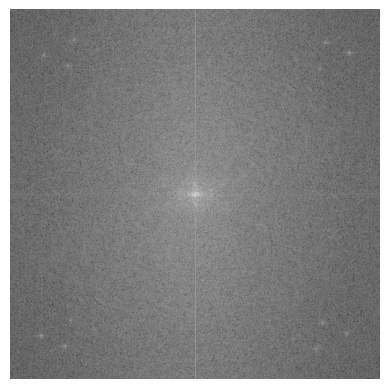
\includegraphics[width=0.3\linewidth]{../resultados/Parte 2/Magnitude.png}
  \caption{Magnitude do espectro centralizado.}
  \label{fig:espec_magnitude}
\end{figure}

\paragraph{Filtro Passa–Baixa}
O filtro passa–baixa preserva apenas as frequências baixas, resultando em um pequeno disco claro no centro do espectro. Na  \href{fig:rec_pb}{imagem reconstruída} é perceptível que a imagem parece mais borrada, causada pela perda de detalhes e uma suavização.

\begin{figure}[H]
  \centering
  \begin{subfigure}[b]{0.45\linewidth}
    \centering
    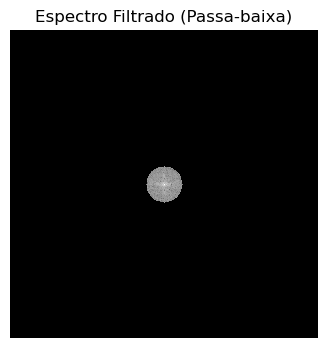
\includegraphics[width=0.7\linewidth]{../resultados/Parte 2/Espectro filtrado passa baixa.png}
    \caption{Espectro filtrado (Passa–Baixa).}
    \label{fig:espec_pb}
  \end{subfigure}
  \hfill
  \begin{subfigure}[b]{0.45\linewidth}
    \centering
    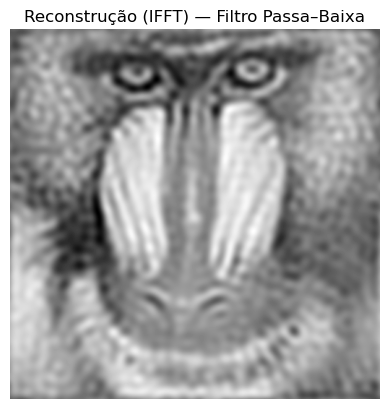
\includegraphics[width=0.7\linewidth]{../resultados/Parte 2/Reconstrução (IFFT) — Filtro Passa–Baixa.png}
    \caption{Reconstrução – Passa–Baixa.}
    \label{fig:rec_pb}
  \end{subfigure}
  \caption{Espectro e reconstrução do filtro passa-baixa.}
  \label{fig:pb_comparacao}
\end{figure}

\paragraph{Filtro Passa–Alta}
O filtro passa–alta atenua as baixas frequências, destacando apenas as altas. No espectro, observa-se um grande disco preto central, e na \href{fig:rec_pa}{imagem reconstruída} predominam bordas e ruídos de alta frequência referente aos pelos do animal que tem uma coloração diferente do seu rosto.

\begin{figure}[H]
  \centering
  \begin{subfigure}[b]{0.45\linewidth}
    \centering
    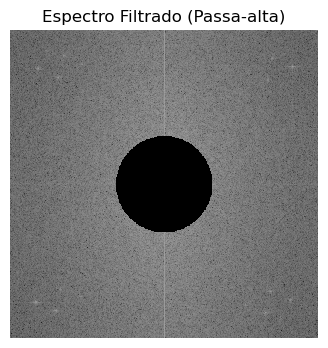
\includegraphics[width=0.7\linewidth]{../resultados/Parte 2/Espectro filtrado passa alta.png}
    \caption{Espectro filtrado (Passa–Alta).}
    \label{fig:espec_pa}
  \end{subfigure}
  \hfill
  \begin{subfigure}[b]{0.45\linewidth}
    \centering
    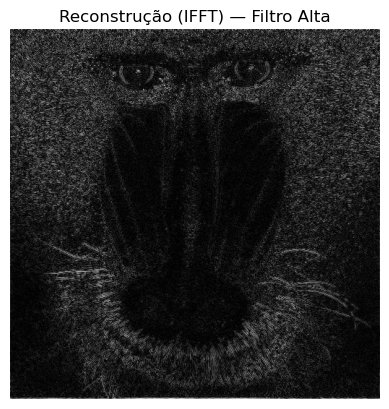
\includegraphics[width=0.7\linewidth]{../resultados/Parte 2/Reconstrução (IFFT) — Filtro Passa–Alta.png}
    \caption{Reconstrução – Passa–Alta.}
    \label{fig:rec_pa}
  \end{subfigure}
  \caption{Espectro e reconstrução do filtro passa-alta.}
  \label{fig:pa_comparacao}
\end{figure}


\paragraph{Filtro Passa–Faixa}
O filtro passa–faixa preserva apenas uma faixa intermediária de frequências, resultando num anel claro no espectro. A \href{fig:rec_pf}{imagem reconstruída} mostra a combinação de suavização e realce.

\begin{figure}[H]
  \centering
  \begin{subfigure}[b]{0.45\linewidth}
    \centering
    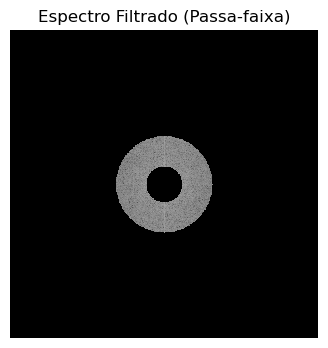
\includegraphics[width=0.7\linewidth]{../resultados/Parte 2/Espectro filtrado passa faixa.png}
    \caption{Espectro filtrado (Passa–Faixa).}
    \label{fig:espec_pf}
  \end{subfigure}
  \hfill
  \begin{subfigure}[b]{0.45\linewidth}
    \centering
    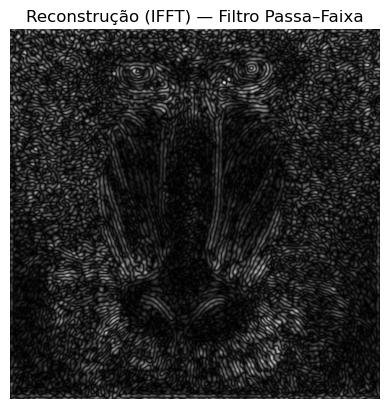
\includegraphics[width=0.7\linewidth]{../resultados/Parte 2/Reconstrução (IFFT) — Filtro Passa–Faixa.png}
    \caption{Reconstrução – Passa–Faixa.}
    \label{fig:rec_pf}
  \end{subfigure}
  \caption{Espectro e reconstrução do filtro passa-faixa.}
  \label{fig:pf_comparacao}
\end{figure}

\paragraph{Filtro Rejeita–Faixa}
O filtro rejeita–faixa elimina frequências intermediárias, deixando apenas baixas e altas. No espectro, podemos ver um anel preto central com região clara interna, e a \href{fig:rec_rf}{imagem reconstruída} exibe simultaneamente suavização com a remoção de algumas bordas referentes ao pêlo do animal.

\begin{figure}[H]
  \centering
  \begin{subfigure}[b]{0.45\linewidth}
    \centering
    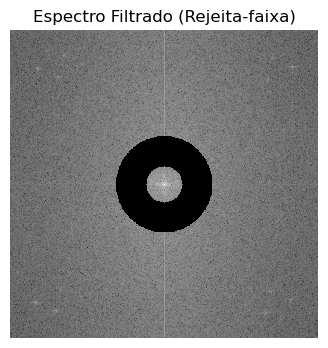
\includegraphics[width=0.7\linewidth]{../resultados/Parte 2/Espectro filtrado rejeita faixa.png}
    \caption{Espectro filtrado (Rejeita–Faixa).}
    \label{fig:espec_rf}
  \end{subfigure}
  \hfill
  \begin{subfigure}[b]{0.45\linewidth}
    \centering
    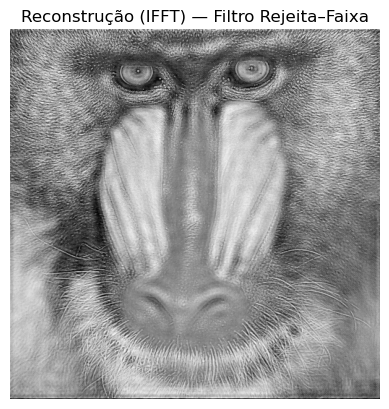
\includegraphics[width=0.7\linewidth]{../resultados/Parte 2/Reconstrução (IFFT) — Filtro Rejeita–Faixa.png}
    \caption{Reconstrução – Rejeita–Faixa.}
    \label{fig:rec_rf}
  \end{subfigure}
  \caption{Espectro e reconstrução do filtro rejeita-faixa.}
  \label{fig:rf_comparacao}
\end{figure}

\paragraph{Compressão por Limiar}
Após aplicar limiar \(T\) e zerar coeficientes de baixa magnitude, a imagem comprimida apresenta redução significativa de detalhes, como mostrado abaixo:

\begin{figure}[H]
  \centering
  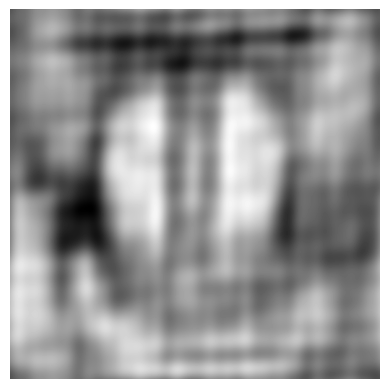
\includegraphics[width=0.3\linewidth]{../resultados/Parte 2/Imagem comprimida.png}
  \caption{Imagem após compressão no domínio de frequência.}
  \label{fig:img_comp}
\end{figure}

\paragraph{Análise do Histograma Comparativo}

Para quantificar o efeito da compressão por limiarização, comparamos os histogramas da imagem original e da comprimida:

\begin{figure}[H]
  \centering
  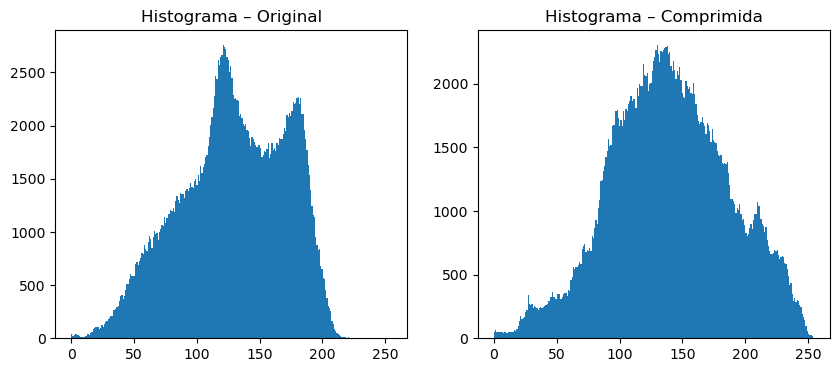
\includegraphics[width=0.8\linewidth]{../resultados/Parte 2/Histograma comparativo.png}
  \caption{Histogramas antes e após compressão por limiar.}
  \label{fig:hist_comp}
\end{figure}

No histograma original observamos uma distribuição com dois picos claros em torno de níveis de cinza 120 e 180. Após a compressão, o histograma apresenta apenas um pico, mostrando que muitos coeficientes de baixa magnitude foram zerados. Esse “achatamento” da distribuição mostra que a compressão remove os detalhes tornando a representação mais uniforme.```

\section{Conclusão}
\paragraph{Para o exercício 1} 
Conseguimos ver como a aplicação dos métodos de difusão de erro utilizando diferentes máscaras e varreduras impacta na qualidade da imagem. Por mais que todas as varreduras apresentem uma certa distorção quanto a imagem original, os resultados mostram que ambas as varreduras preservaram bem os detalhes da imagem original.

\paragraph{Para o exercício 2} 
Conseguimos ver a aplicação de cada filtro no domínio da frequência, e como eles afetam a imagem original. Causando suavização, realce ou compressão. Além disso, realizar a compressão por limiarização mostrou como eliminar os coeficientes de baixa magnitude torna a imagem mais uniforme, causando perda de detalhes.


\end{document}